% Original course content. Uses unmodified zju_beamer.sty by its credited authors.
% Theme source pinned at qychen2001/ZJU-Beamer-Template a276635341cee0e5b31c5ac004a1999fb3c9785b.
\PassOptionsToPackage{quiet}{fontspec}
\PassOptionsToPackage{dvipsnames}{xcolor}
\documentclass[10pt,aspectratio=169]{beamer}
\usepackage{zju_beamer}
\usepackage{booktabs}
\graphicspath{{./figures/}}
\zjusectioncolor{blue}
\title[二维多孔导热]{气凝胶启发的二维多孔介质导热预测}
\subtitle{物理模型、机器学习与混合模型的适用边界}
\author[课程汇报]{汇报人：\underline{\hspace{2cm}}}
\institute[化工学院]{化学工程与生物工程学院\\浙江大学}
\date[2026年10月]{2026年10月}
\newcommand{\source}[1]{\par\vspace{1mm}{\scriptsize #1}}
\newcommand{\resultplot}[1]{\centering\includegraphics[width=.82\textwidth,height=.65\textheight,keepaspectratio]{#1}}
\begin{document}
\begin{frame}\titlepage\end{frame}
\section{问题}
\begin{frame}{孔隙率相同，导热路径可以不同}
\begin{columns}[T]
\column{.55\textwidth}
\begin{itemize}
\item 气凝胶及多孔绝热材料具有复杂骨架与方向关系\cite{abraham2023,wei2020}。
\item 有效介质模型用相比例近似空间结构。
\item 新结构是否仍处于模型可信预测域？
\end{itemize}
\column{.42\textwidth}
\begin{block}{本工作的问题}
哪些结构信息改善预测？\\[2mm]
Physics、RF、残差Hybrid在什么区域误差较低？
\end{block}
\end{columns}
\source{研究对象：合成二维复杂多孔结构；不是实验气凝胶微结构。}
\end{frame}
\section{方法}
\begin{frame}{360幅图像对应180个母结构}
\begin{itemize}
\item 高斯相关场阈值化，$64\times64$二值图。
\item fine、coarse、anisotropic三个生成族。
\item $\phi=0.30,0.45,0.60,0.75,0.90$；每组合12母结构。
\item 原图与$90^\circ$旋转成对，按母结构分组。
\end{itemize}
\begin{block}{两条独立计算路径}
几何$\rightarrow$9项结构描述符；几何$\rightarrow$FVM数值标签。\\
描述符不读取温度、热流或真实$k$。
\end{block}
\end{frame}
\begin{frame}{FVM标签来自传热方程}
\[\nabla\!\cdot[k(x,y)\nabla T]=0\]
\begin{columns}[T]
\column{.52\textwidth}
\begin{itemize}
\item 左$T=1$、右$T=0$；上下绝热。
\item $k_s=100$、$k_p=1$；$128\times128$网格。
\item 界面谐均面导热率，控制体守恒。
\end{itemize}
\column{.43\textwidth}
\[k_{eff}=\frac{Q L}{W\Delta T}\]
均匀相、串并联解析解检查；30例网格细化。\\[2mm]
128与256格相对差：中位0.608\%，最大1.962\%。
\end{columns}
\source{数值参考属于当前二维方程；误差单位是无量纲$k/k_p$\cite{patankar1980}。}
\end{frame}
\begin{frame}{同一母结构的两个方向}
\begin{columns}[T]
\column{.46\textwidth}\centering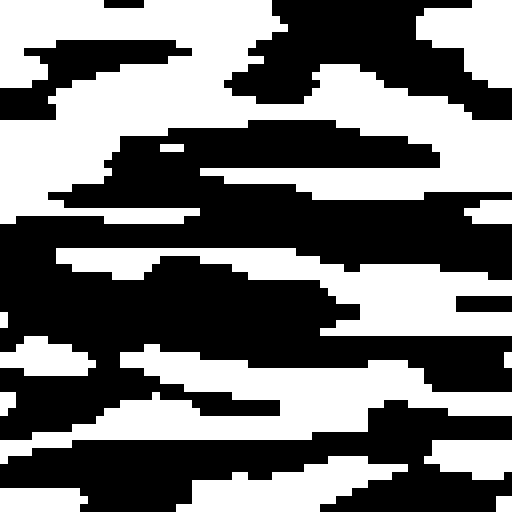
\includegraphics[height=.54\textheight]{pair0.png}\\$k_{FVM}=32.409$
\column{.46\textwidth}\centering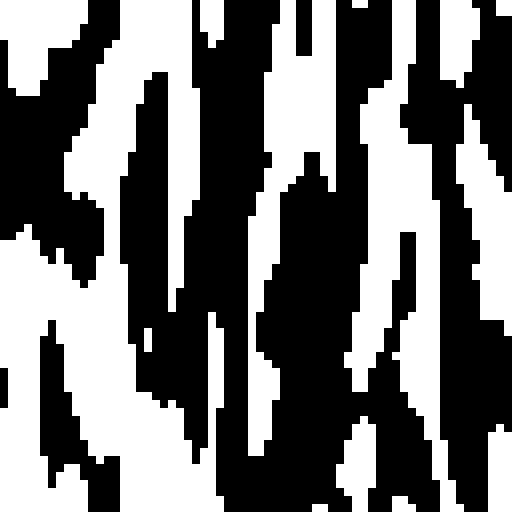
\includegraphics[height=.54\textheight]{pair1.png}\\$k_{FVM}=4.810$
\end{columns}
\vspace{2mm}\centering
相同$\phi$；孔隙率Physics两方向均约16.115。
\source{固相黑、孔相白；热流水平。旋转对不跨训练与测试。}
\end{frame}
\begin{frame}{物理基线与训练集校准}
\[(1-\phi)\frac{k_s-k}{k_s+k}+\phi\frac{k_p-k}{k_p+k}=0\]
\begin{itemize}
\item 原Physics：二维Bruggeman，$a=1$\cite{bruggeman1935}。
\item 1p校准：分母$k\rightarrow ak$，训练集拟合全局$a$。
\item 3p结构：$a=\exp\{\mathrm{clip}[\theta_0+\theta_1 A+\theta_2(B-0.5),-4,4]\}$。
\end{itemize}
$A$为方向参数，$B$为瓶颈；3p是半经验形状控制\cite{lu2022}。\\
校准排除“原参数未标定好”的混淆，测试标签不参与拟合。
\end{frame}
\begin{frame}{RF直接预测与Hybrid残差学习}
\begin{columns}[T]
\column{.48\textwidth}
\begin{block}{Pure RF}
9项几何描述符$\rightarrow k_{FVM}$\\[2mm]
128树、叶至少3样本、单CPU线程\cite{breiman2001}。
\end{block}
\column{.48\textwidth}
\begin{block}{Physics + residual RF}
$r_{train}=k_{FVM}-k_{Physics,cal}$\\[2mm]
$\hat k_{Hybrid}=k_{Physics,cal}+\hat r_{RF}$
\end{block}
\end{columns}
\vspace{3mm}
相同输入、相同RF容量；差别是学习目标。\\
没有PDE损失或硬守恒约束，本文Hybrid不是PINN。
\end{frame}
\begin{frame}{按预测区域验证，而非只做随机划分}
\begin{tabular}{lll}\toprule
区域&训练与测试&重复含义\\\midrule
同分布&144/36母结构&10个group split\\
中间缺口&留出整个$\phi=0.60$&固定区域、10森林seed\\
高$\phi$外推&训练$\phi\leq0.75$，测试0.90&同上\\
未见族&fine/coarse训练，anisotropic测试&同上\\\bottomrule
\end{tabular}
\par\vspace{3mm}
训练池25/50/75/100\%嵌套；测试组不变。\\
报告MAE、RMSE、$R^2$；森林seed波动不是10个独立OOD试验。
\end{frame}
\section{结果}
\begin{frame}{全结构RF误差降低，孔尺度统计没有改善}
\resultplot{ablation.pdf}
\source{10次分组留出，mean$\pm$SD。贯通、方向和截面路径提供主要增益；历史5split结果单独保留。}
\end{frame}
\begin{frame}{同分布：RF与Hybrid平均误差接近}
\resultplot{iid.pdf}
\source{RF：$1.657\pm0.243$；Hybrid：$1.684\pm0.298$。约0.027差异不支持稳定优劣，也不是等效性证明。}
\end{frame}
\begin{frame}{没有稳定的小数据Hybrid优势}
\resultplot{learning.pdf}
\source{25/50/75/100\%训练池，10次分组留出；75\%档微小优势没有形成一致趋势。}
\end{frame}
\begin{frame}{未见中间$\phi=0.60$：Hybrid误差较低}
\resultplot{middle.pdf}
\source{RF 2.888；Hybrid 1.417。属于$\phi$范围内的数据缺口，不是对所有插值或OOD的保证。}
\end{frame}
\begin{frame}{高$\phi=0.90$外推：解析相极限更可靠}
\resultplot{high.pdf}
\source{Physics 0.125；RF 0.897；Hybrid 0.391。原Physics的$R^2$仍为$-0.319$，负值保留。}
\end{frame}
\begin{frame}{RF训练标签下界与残差迁移偏差}
\begin{columns}[T]
\column{.48\textwidth}
\begin{block}{RF}
训练标签最小约1.525，测试最小约1.150。\\[2mm]
叶均值无法低于训练标签下界；首seed预测均值约2.246。
\end{block}
\column{.48\textwidth}
\begin{block}{Hybrid}
真实残差均值约0.121；学习修正均值约0.521。\\[2mm]
物理主干有相极限，但额外修正偏大。
\end{block}
\end{columns}
\source{固定高$\phi$区域、首seed诊断；不外推为所有物理/ML问题的机制定律。}
\end{frame}
\begin{frame}{未见各向异性族：3p结构Physics较好}
\resultplot{family.pdf}
\source{3p 3.175；RF 4.512；Hybrid 4.937；原Physics 8.254。需要区分结构物理与孔隙率物理。}
\end{frame}
\section{讨论}
\begin{frame}{残差可以学习，Hybrid仍未全面获益}
\begin{itemize}
\item 同分布残差RF测试$R^2\approx0.873$。
\item 校准Physics误差4.835，Hybrid降至1.684。
\item 直接RF已读取相同结构；追加Physics为第10输入，MAE 1.655。
\item 同分布出现1次负预测、3次物理界限越界，含重复测试样本，未裁剪。
\end{itemize}
\source{物理主干是归纳偏置，不自动增加几何信息，也不自动约束总输出。}
\end{frame}
\begin{frame}{模型适用域取决于物理关系和数据覆盖}
\begin{tabular}{ll}\toprule
当前目标域&本数据中较低误差模型\\\midrule
同生成族/已采样层&全结构RF；Hybrid接近\\
中间$\phi$缺口&Hybrid\\
孔相主导的高$\phi$相极限&低参数Physics\\
未见方向族&包含方向关系的3p Physics\\\bottomrule
\end{tabular}
\par\vspace{4mm}
没有统一冠军模型。未知材料或缺失物理机制时，这张表不能替代新参考数据。
\end{frame}
\begin{frame}{真实气凝胶检查尚不能验证迁移}
\begin{itemize}
\item 筛查73条/17论文组，实测孔隙率仅34条/8组\cite{walker2023}。
\item pooled相关：密度约0.618，孔隙率约$-0.448$。
\item 测量温压缺失、体系混杂，无贯通/方向图像。
\item 当前不含3D、Knudsen、辐射、接触和条件依赖。
\end{itemize}
\source{这是有限趋势与现实距离，不是严格外部验证；没有重新训练实验模型。}
\end{frame}
\begin{frame}{AI的主要瓶颈是可信域识别}
\begin{itemize}
\item 180母结构、三个生成族，不能代表全部材料形貌。
\item 描述符和数值模型遗漏机制，复杂网络不能自动补齐。
\item 随机划分可能掩盖来源/结构迁移问题。
\item 轻量距离告警：IID 7.5\%，高$\phi$ 52.8\%，未见族100\%。
\end{itemize}
\begin{block}{Level 3依据}
FVM + 有效介质物理 + 结构知识 + RF/残差结合 + 适用域检验。\\
Hybrid不必全面胜出；树间SD在高$\phi$全部漏判，距离提示也有限。
\end{block}
\end{frame}
\section{复现}
\begin{frame}[fragile]{M4 CPU即可完整复现}
\begin{lstlisting}[language=python]
python scripts/run_all.py
\end{lstlisting}
\begin{itemize}
\item MacBook Air M4，macOS，Python3.12.14，CPU。
\item GitHub新clone重算38.6秒；9测试，49行指标/70计划一致。
\item \url{https://github.com/Forever61T/porous-thermal-ai}
\item v1.0.0主指标冻结；v1.1.0候选含轻量OOD诊断，无CNN。
\end{itemize}
\source{38.6秒为原主流程历史实测，不含安装；候选新增2项隔离测试，共11项。}
\end{frame}
\section{文献}
\begin{frame}[allowframebreaks]{参考文献}\footnotesize\reference\end{frame}
\end{document}
